% Standalone source for Figure 1 (FreqLite architecture).
% Compile to a cropped PDF used by the manuscript via \includegraphics:
%   pdflatex architecture.tex   ->  architecture.pdf
% (copy/move the result to ../results/figures/architecture.pdf)
\documentclass[border=2pt]{standalone}
\usepackage{amsmath,amssymb,amsfonts}
\usepackage{tikz}
\usetikzlibrary{positioning,calc,arrows.meta,fit,backgrounds}
\newcommand{\method}{\textsc{FreqLite}}
\newcommand{\bs}{\mathbf{s}}
\newcommand{\by}{\mathbf{y}}
\newcommand{\R}{\mathbb{R}}
\begin{document}
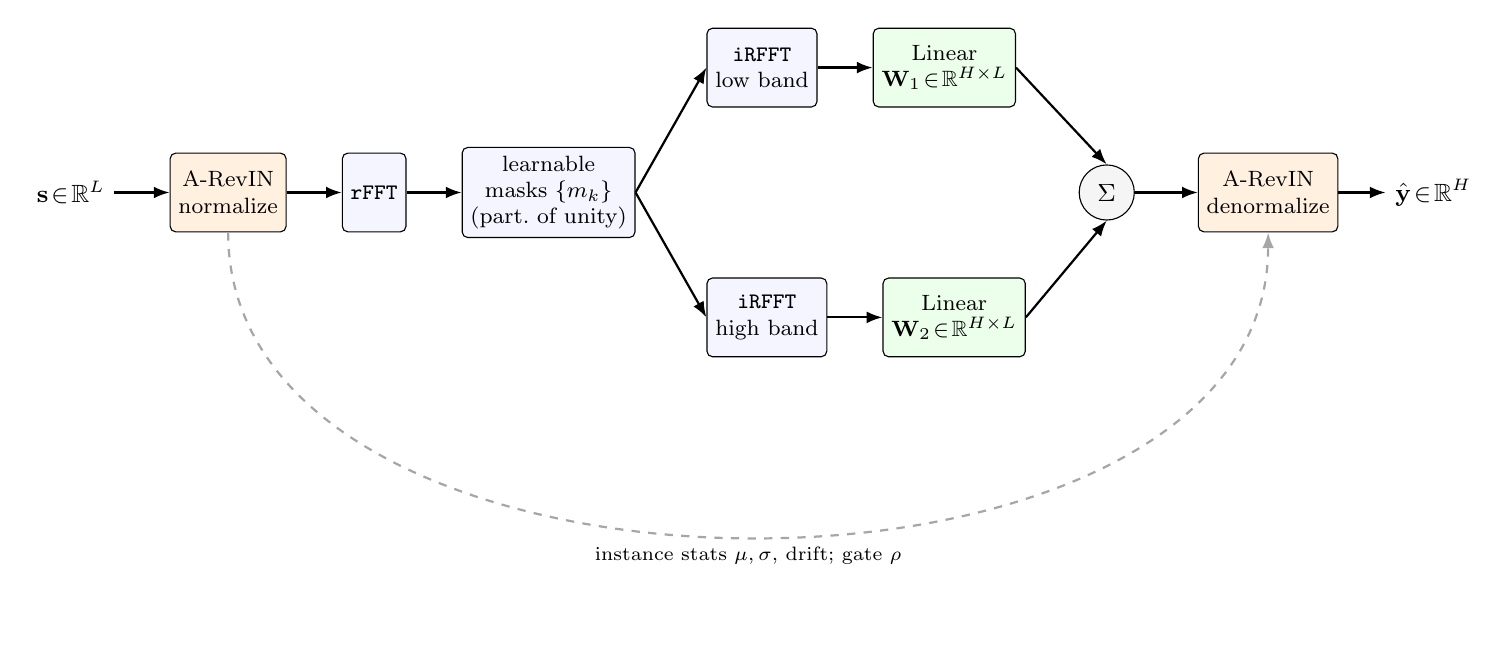
\begin{tikzpicture}[
    >={Latex[length=2mm]},
    node distance=6mm and 7mm,
    box/.style={draw, rounded corners=2pt, minimum height=10mm, align=center,
                font=\footnotesize, inner sep=3pt, fill=blue!4},
    norm/.style={box, fill=orange!12},
    head/.style={box, fill=green!8},
    op/.style={draw, circle, minimum size=7mm, font=\small, inner sep=0pt, fill=gray!8},
    io/.style={font=\small\itshape},
    arr/.style={->, thick},
  ]
    \node[io] (in) {$\bs\!\in\!\R^{L}$};
    \node[norm, right=of in]   (nrm)  {A-RevIN\\normalize};
    \node[box,  right=of nrm]  (fft)  {\texttt{rFFT}};
    \node[box,  right=of fft]  (mask) {learnable\\masks $\{m_k\}$\\(part.\ of unity)};
    \node[box,  above right=5mm and 9mm of mask] (irL)  {\texttt{iRFFT}\\low band};
    \node[box,  below right=5mm and 9mm of mask] (irH)  {\texttt{iRFFT}\\high band};
    \node[head, right=of irL]  (linL) {Linear\\$\mathbf{W}_1\!\in\!\R^{H\times L}$};
    \node[head, right=of irH]  (linH) {Linear\\$\mathbf{W}_2\!\in\!\R^{H\times L}$};
    \node[op] (sum) at ($(linL)!0.5!(linH)+(2.0cm,0)$) {$\Sigma$};
    \node[norm, right=8mm of sum] (dn) {A-RevIN\\denormalize};
    \node[io, right=6mm of dn] (out) {$\hat{\by}\!\in\!\R^{H}$};
    \draw[arr] (in) -- (nrm);
    \draw[arr] (nrm) -- (fft);
    \draw[arr] (fft) -- (mask);
    \draw[arr] (mask.east) -- (irL.west);
    \draw[arr] (mask.east) -- (irH.west);
    \draw[arr] (irL) -- (linL);
    \draw[arr] (irH) -- (linH);
    \draw[arr] (linL.east) -- (sum.north);
    \draw[arr] (linH.east) -- (sum.south);
    \draw[arr] (sum) -- (dn);
    \draw[arr] (dn) -- (out);
    \draw[->, thick, dashed, gray!70]
      (nrm.south) to[out=-90,in=-90]
      node[below, font=\scriptsize, text=black, midway]
      {instance stats $\mu,\sigma$, drift; gate $\rho$}
      (dn.south);
\end{tikzpicture}
\end{document}
